\hspace{3mm}

\begin{wrapfigure}{r}{0.25\linewidth}
    \centering
    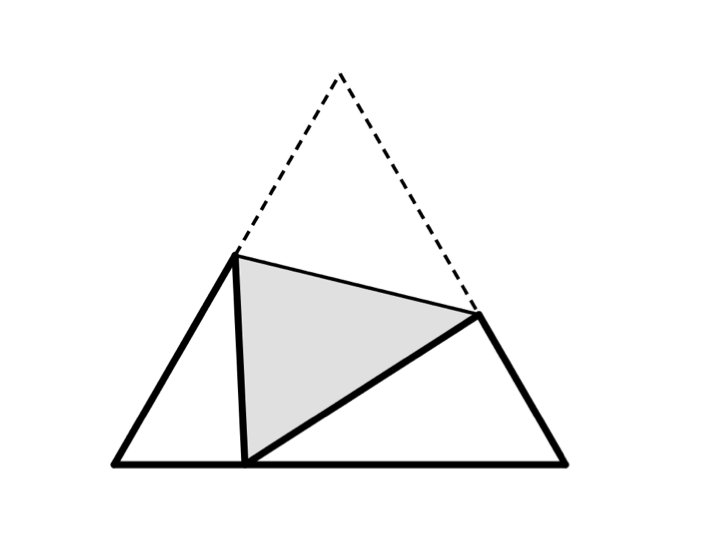
\includegraphics[width=\linewidth]{ЭлМШ 2023-2024/VII блок/Киви/lesson_1/Task_1.png}
\end{wrapfigure}

\centerline{\Huge \bf  Движения плоскости}
\centerline{\Huge \bf Центральная и осевая симметрии}

\begin{flushright}
    \scriptsize{}
\end{flushright}

\hspace{3mm}

\problem{1} Бумажный равносторонний треугольник перегнули по прямой так, что одна из вершин попала на противоположную сторону (см. рисунок). Докажите, что углы двух белых треугольников соответственно равны.

\problem{2} На продолжении диагонали $AC$ квадрата $ABCD$ за точку $C$ выбрана точка $X$ так, что $BX$ = $AC$. Найдите угол $\angle AXB$

\problem{3} На диагонали $AC$ квадрата $ABCD$ выбраны точки $XY$ и $Y$ так, что точка $Y$ лежит на отрезке $CX$ и $XY = YD$. Известно, что $\angle XBC = \alpha $. Чему равен $\angle XYD$?

\begin{wrapfigure}{r}{0.2\linewidth}
    \centering
    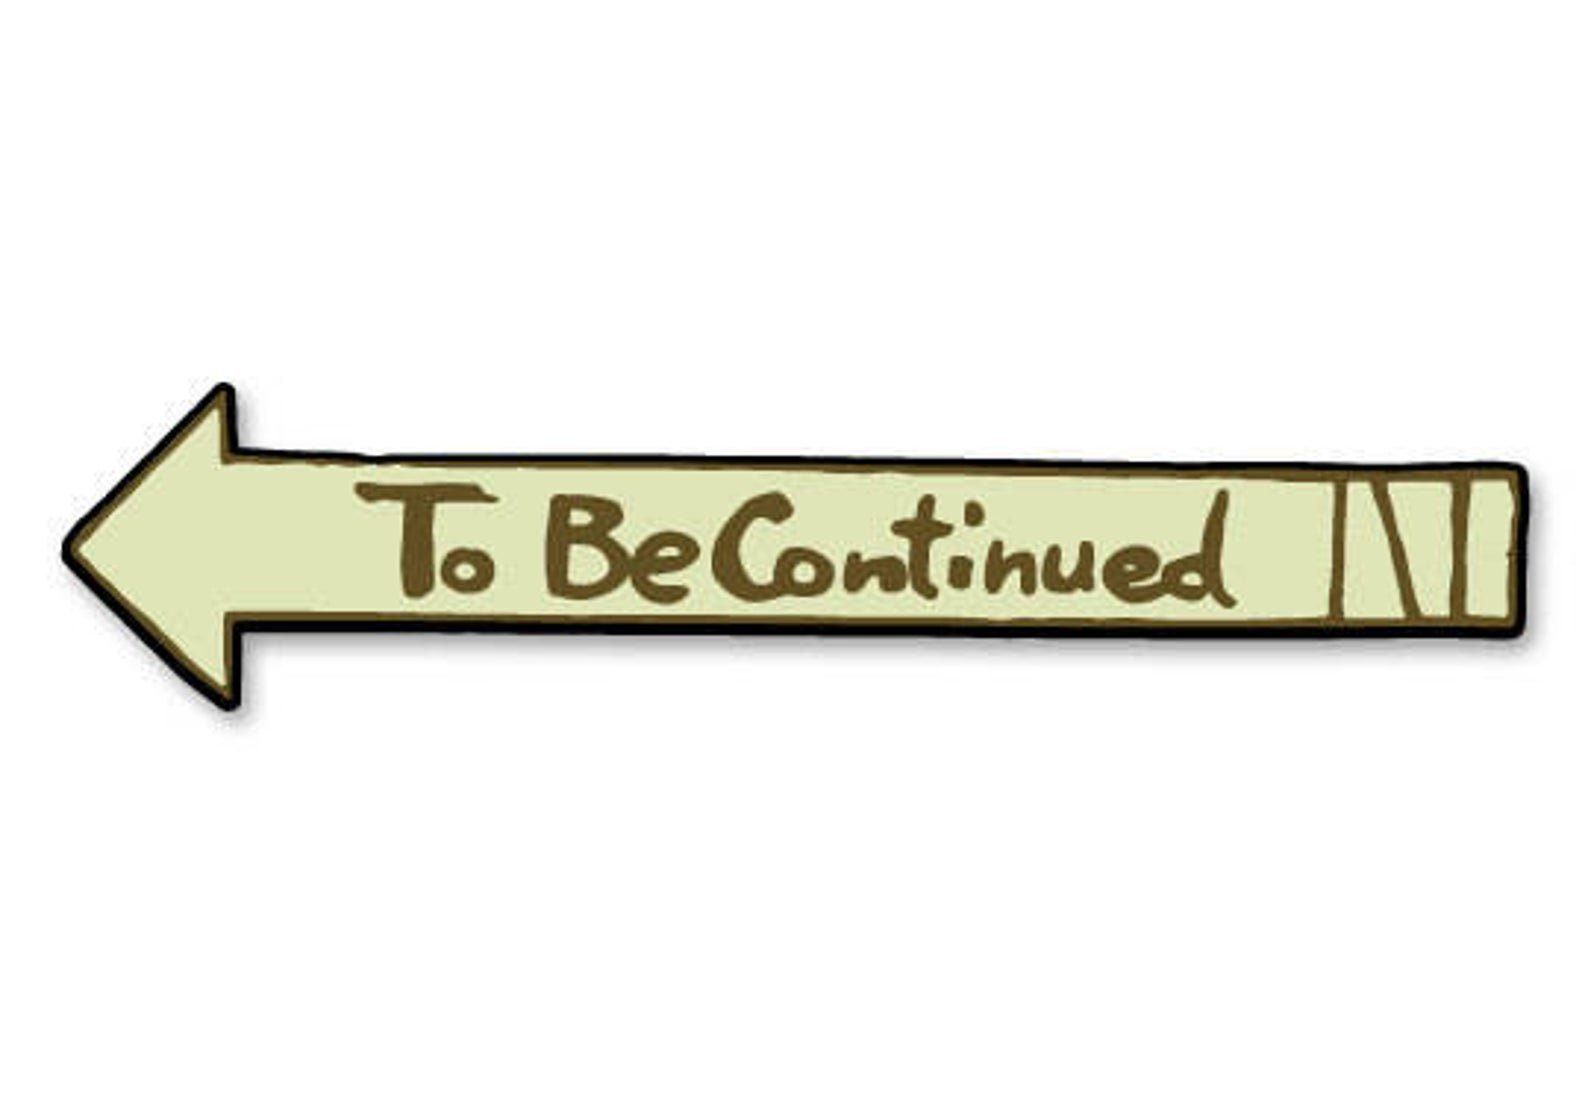
\includegraphics[width=\linewidth]{ЭлМШ 2023-2024/VII блок/Киви/lesson_1/to_be_continued.jpeg}
\end{wrapfigure}

\problem{4} На стороне $BC$ треугольника $ABC$ выбрали точки $P$ и $Q$ такие, что $BA$ = $BP$ и $CA = CQ$ . Точка $I \ -$  точка пересечения биссектрис треугольника $ABC$. Докажите, что треугольник $IPQ$ равнобедренный.

\problem{5}
а) \textit{Теорема об угле между биссектрисами.} Докажите, что сторона $BC$ треугольника $ABC$ видна из центра $O$ вписанной окружности под углом $90^{\circ}+\angle A/2$.

\noindentб$)^{*}$ Биссектрисы треугольника $ABC$ пересекаются в точке $I$,  $\angle ABC = 120^{\circ}.$ На продолжениях сторон $AB$ и $CB$ за точку $B$ отмечены соответственно точки $P$ и $Q$ так, что  $SP = CQ = AC$.  Докажите, что угол $PIQ$ - прямой. 

\textit{Подсказка:} воспользуйтесь теоремой об угле между биссектрисами.
%https://problems.ru/view_problem_details_new.php?id=117007

\centerline{\Large \bf Центральная симметрия.}

\problem{6} На прямоугольном торте лежит круглая печенька Oreo. Как разрезать торт на две равные части так, чтобы и печенька тоже разделилась ровно пополам?

\textit{Подсказка:} Если фигура имеет центр симметри, то любая прямая проходящая через него делит фигуру пополам.

\problem{7} В четырёхугольнике $ABCD$ точки $K,\ L,\ M,\ N -$ середины сторон соответственно $AB,  BC,\  CD,\  DA$. Прямые AL и CK пересекаются в точке $P$, прямые $AM$ и $CN -$ пересекаются в точке $Q$. Оказалось, что $APCQ - $ параллелограмм. Докажите, что $ABCD\ -$ тоже параллелограмм.